% This version of CVPR template is provided by Ming-Ming Cheng.
% Please leave an issue if you found a bug:
% https://github.com/MCG-NKU/CVPR_Template.

\documentclass[review]{cvpr}
%\documentclass[final]{cvpr}

\usepackage{times}
\usepackage{epsfig}
\usepackage{graphicx}
\usepackage{amsmath}
\usepackage{amssymb}

% Include other packages here, before hyperref.

% If you comment hyperref and then uncomment it, you should delete
% egpaper.aux before re-running latex.  (Or just hit 'q' on the first latex
% run, let it finish, and you should be clear).
\usepackage[pagebackref=true,breaklinks=true,colorlinks,bookmarks=false]{hyperref}


\def\cvprPaperID{****} % *** Enter the CVPR Paper ID here
\def\confYear{CVPR 2021}
%\setcounter{page}{4321} % For final version only


\begin{document}

%%%%%%%%% TITLE
\title{Forging Handwritten Signatures}

\author{Andrew Fryer\\
Queen's University\\
99 University Ave, Kingston, ON, Canada\\
{\tt\small andrew.fryer@queensu.ca}
% For a paper whose authors are all at the same institution,
% omit the following lines up until the closing ``}''.
% Additional authors and addresses can be added with ``\and'',
% just like the second author.
% To save space, use either the email address or home page, not both
\and
Second Author\\
Institution2\\
First line of institution2 address\\
{\tt\small secondauthor@i2.org}
}

\maketitle


%%%%%%%%% ABSTRACT
\begin{abstract}
% -verification is...
% -facenet is...
% -Signet is...
% -we want to forge...
% -FGSM is...
% -we got good/bad results using _ training set up
   The ABSTRACT is to be in fully-justified italicized text, at the top
   of the left-hand column, below the author and affiliation
   information. Use the word ``Abstract'' as the title, in 12-point
   Times, boldface type, centered relative to the column, initially
   capitalized. The abstract is to be in 10-point, single-spaced type.
   Leave two blank lines after the Abstract, then begin the main text.
   Look at previous CVPR abstracts to get a feel for style and length.
\end{abstract}

%%%%%%%%% BODY TEXT
\section{Introduction}\label{sec:introduction}

Verfying people's identity (I think it is call authentication in security circles...) is a difficult problem...

Handwritten signatures have been used for verifying people's identity for a long time.

Face verification from images is an old problem.

``Offline signature verification is one of the most challenging tasks in biometrics and document forensics. Unlike other verification problems, it needs to model minute but critical details between genuine
and forged signatures, because a skilled falsification might only differ from a real signature by some
specific kinds of deformation. This verification task is even harder in writer independent scenarios
which is undeniably fiscal for realistic cases. In this paper, we model an offline writer independent
signature verification task with a convolutional Siamese network.''\cite{sig_net}

This could be done by training a CNN to output whether or not the input image is of the chosen person.
However, this requires a new network to be trained for each person that the system needs to perform verification for.
Not only is it computationally very expensive to train such a system to perform verification for many people, but also requires a large number of images of the person's face for training.

Instead, a high-level representation of the image can be found that includes only the information needed to distinguish people.
This is effectively dimensionality reduction that preserves only the information that is important for identifying people.
The high-level representation is a vector in what is reffered to as a latent space.
(So, the dimensionality reduction should preserve/extract the structure of the person's face while discarding information about the background and the lighting conditions.)
Then,

``The existence of adversarial examples suggests that being able to
explain the training data or even being able to correctly label the test data does not imply that our
models truly understand the tasks we have asked them to perform. Instead, their linear responses are
overly confident at points that do not occur in the data distribution, and these confident predictions
are often highly incorrect''\cite{goodfellow}.


\section{Related Work}\label{sec:related_work}

\subsection{Before CNNs} % todo: rename
``Handwriting was developed a long time ago as a means to expand human memory and to facilitate communication''\cite{handwriting_survey}.
``Handwriting is a skill that is personal to individuals''\cite{handwriting_survey}.

``in numerous situations, a pen together with paper or a small notepad is more convenient that a keyboard''\cite{handwriting_survey}.
Early research in to machine recognition of handwriting was motiviated by the desire to allow humans to write conveniently and then parse that writing into data inside of a computer.
On-line: 2-D coordinates as a function of time. (captured by electronic device)
Off-line: image. (usually captured using paper)
\cite{handwriting_survey}
As of [year], on-line handwriting recognition was more accurate than off-line recognition because the extra information is useful.
``recognition rates reported are much highter for the on-line case in comparison with the off-line case''
Personal Digital Assistants (PDAs) use on-line systems have been used widely commercially.
These techniques worked like so...
    Structural and rule-based methods, statistical methods, implicit methods (artificiall neural networks)
    Hidden Markov Model process
One of these techniques used a CNN and HMM\cite{389575}.
This work was built off of LeCun's early work on CNNs.
None of these methods have been accurate enough to be used commercially on cursive writing.
However, off-line handwriting recognition is much more broadly applicable because it does not require a special device to capture the handwriting.
Only a camera is needed to capture an image of the writing.
There have been several attempts made to recreate the temporal data from an image, but these have not been very successful.\cite{handwriting_survey}.

``Handwriting interpretation is the task of determining the meaning of a body of handwriting''\cite{handwriting_survey}.
``Handwriting identification is the the task of determining the autor of a sample of handwriting form a set of writers, assuming that each person's handwriting is individualistic. Signature verificiation is the task of determining whether or not the signature is that of a given person''\cite{handwriting_survey}.
Verfication attempts to extract the writer-specific information from a signature ``irrespective of its handwritten content''.
A bank might require an error of 1/ 100,000. ``Current systems are sill several orders of magnitude away''.

\subsection{MNIST/LeCun}
In 1998, LeCun famously tackled the problem of off-line handwritten digit recognition using [i think a new technique] convolutional neural networks\cite{mnist}.


\subsection{Contrastive Loss}
``The idea of mapping face images to low dimensional target spaces before comparison has a long history''
``Our approach is to build a trainable system that nonlinearly maps the raw images of faces to points in a low dimensional space so that the distance between these points is
small if the images belong to the same person and large otherwise. Learning the similarity metric is realized by training a network that consists of two identical convolutional
networks that share the same set of weights - a Siamese Architecture''
\begin{figure}[h]
    \begin{center}
        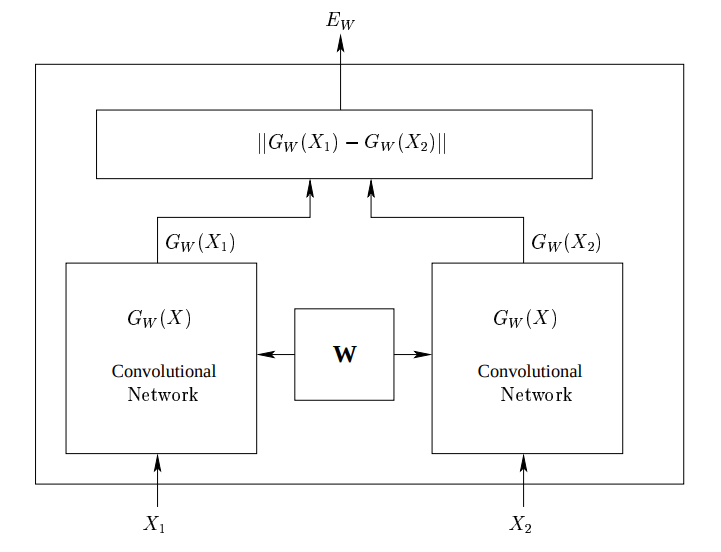
\includegraphics[width=0.8\linewidth]{siamese_architecture.png}
    \end{center}
    \caption{Siamese Architecture. (LeCun 2005)}
    \label{fig:siamese}
\end{figure}
I think LeCun proposed Contrastive Loss...\cite{LeCun}.
[Note: the partitioning and pairing of images is the same idea as SigNet.]
They did this on images of faces.

``A model is constructed of each subject by calculating the mean feature
vector and the variance-covariance matrix using the feature
vectors generated from the first five images of each subject.
The likelihood that a test image is genuine, $p_genuine$, is
found by evaluating the normal density of the test image on
the model of the concerned subject. The likelihood of a test
image being an impostor, $p_imposter$, is assumed to be a constant whose value is estimated by calculating the average $p_genuine$ value of all the impostor images of the concerned
subject. The probability that the given image is genuine is
given by P = $p_genuine$ / ($p_genuine$ + $p_imposter$)''
...so basically they assume that subjects/signers occupy a normal region in the latent space.

\subsection{Triplet Loss}
``FaceNet directly trains
its output to be a compact 128-D embedding using a triplet-based loss function based on LMNN [19]. Our triplets consist of two matching face thumbnails and a non-matching
face thumbnail and the loss aims to separate the positive pair
from the negative by a distance margin. The thumbnails are
tight crops of the face area, no 2D or 3D alignment, other
than scale and translation is performed.''
You could train a classifier and then take an intermediate layer to be a latent space, but this doesn't perform as well...
PCA can improve this, but an end-to-end network performs better.
\cite{face_net}

`` The networks are trained by using a combination of classification and verification loss. The verification
loss is similar to the triplet loss we employ [12, 19], in that it
minimizes the L2-distance between faces of the same identity and enforces a margin between the distance of faces of
different identities. The main difference is that only pairs of
images are compared, whereas the triplet loss encourages a
relative distance constraint.''
``Although we did not directly compare to other losses,
e.g. the one using pairs of positives and negatives, as used
in [14] Eq. (2), we believe that the triplet loss is more suitable for face verification. The motivation is that the loss
from [14] encourages all faces of one identity to be projected onto a single point in the embedding space. The
triplet loss, however, tries to enforce a margin between each
pair of faces from one person to all other faces. This allows the faces for one identity to live on a manifold, while
still enforcing the distance and thus discriminability to other
identities.''
When training, they don't use true negatives to adjust weights because the network already knows they are different and so the direction of the gradient is somewhat arbitrary...
[Maybe I should try that...]
They just use a cut off threshold for computing accuracy.
Part of the results of their paper is that they comclude that using 256-bit over 128-bit latent vectos doesn't really improve accuracy.


\subsection{SigNet}
SigNet was largely inspired by the success of FaceNet.
I haven't seen the SigNet paper discuss why they didn't use triplet loss...

Yo, why does SigNet use contrastive loss instead of triplet loss?
    My guess is that Contrastive Loss is just easier to implement...
\cite{sig_net}
\cite{GitHub_sounakdey}
...and in python: \cite{GitHub_signet_pytorch}

\subsection{DeepFool}
\subsection{DEFENSE-GAN}

\subsection{FGSM}



\section{Implementation}\label{sec:implementation}

Take Signet.
Attack it using a technique similar to FGSM.
[Try to improve SigNet's resilience to the attack.]

% TODO: divide this into subsections

For implementing the SigNet, 3 resources were used.
The SigNet paper was consulted, which describes the model completely\cite{sig_net}.
The Keras code presumably by one of the paper authors was used for clarification\cite{GitHub_sounakdey}.
Lastly, an existing PyTorch implementation of SigNet was used as a starting place\cite{GitHub_signet_pytorch}.

The existing PyTorch implementation first restructured into a Jupyter Notebook.
Then, it was checked against the specification of the network in the paper.
The existing training process did not implement data normalization, so this was implemented as per the paper.
The mean and standard deviation of the images in the training dataset was computed (after spliting the images in the CEDAR dataset into training and validation images and pairing images).
For efficiency, all of the images in the dataset were then resized, transformed (inverted), and normalized according the paper's description and then saved back into png files.
[I didn't save the image data to disk as a .pt file (as a tensor) because I figured that png compression is probably better than the .pt compression since it is image-specific.]

Unfortunately, it was later discovered that the last layer of the network was incorrect in the existing implementation and this went unnoticed.
The Signet implementation in this paper has [last layer output size is 256 instead of 128].
% would training go faster if this was fixed?
% I could also try to use the trained incorrect model to initialize the correct model...

The process of preparing the data is all the same.
While the paper uses several datasets, this paper only uses the CEDAR dataset due to time constraints [ref].
% todo: ref

Another small disrepency is in the initialization of model weights.
% todo
% I'm not sure if the biases were correctly initialized to 0 or if the other weights were initialized with the same strategy...

Training was done on Google Colab (using the \_ level tier thing).
The training process took approximately 1 hour per 1000 [cases/datapoints].
The training process was changed to use a dataloader that stores all of the image data in computer memory instead of repeatedly accessing the information from disk in the form of PNG files.
This is feasible because the number of images is far fewer than the number of pairs of images (which are used as [cases/datapoints]).
Unfortunately, this did not seem to speed up the training process significantly.

I should try increasing the batch size!!!!

The model was trained for approximately \_ hours [until batch 19050] and then evaluated, yeilding an accuracy of 72\%.
Then, it was trained until the end of the first epoch (another \_ hours) and evaluated [validated?] again.
This time the accuracy was 94\%.

Although the paper trains the model for 20 epochs, training was stopped at 1 epoch due to time constraints and because 94\% accuracy seemed sufficient for the puposes of this paper.
(Unfortuantely weights from a trained SigNet model could not be obtained.)

% \section{Expirements}
The code in the repo presumably by the SigNet paper author computes accuracy given a thrsehold that is determined by taking the threshold that gives the best accuracy on the validation set.
IMHO, this is wrong because the threshold is information that is technically part of the classifier that is being leaked from the validation set.
See: \url{https://github.com/sounakdey/SigNet/blob/master/SigNet_v1.py#L84}
This approach is useful for understanding the potential of SigNet, but does not give an accuracy evaluation of the accuracy that SigNet would have in the real world because of this information leakage.


I should compute the divide as $p_same / (p_same + p_different)$ where each p is computed as the gaussian distribution of the distances on the training data...

!!! I don't think that SigNet implements the decision (genuine vs. forge) correctly !!!
It treats all dimensions with equal weight, whereas LeCun computes the mean and cov mat of several genuine images and then computes p based on a gaussian/normal assumption.
Yeah, SigNet just finds a threshold distance and uses that... (which naively weights all dimensions equally)

I think that what I should implement (also) is compute the mean and covariance (matices) of the genuine and forge data latent vectors over a bunch of training pairs. (To compute variance, I might need to store the latent vectors in CPU RAM and free the GPU RAM to avoid GPU OOM.)
I can also compute the confusion matrix using the simple threshold distance and my thing and discuss the performance differences.

Maybe I should also try what LeCun did with computing normal distribution for an individual and then using inverse FGSM (aka gradient descent on the input... could I use Pytorch optimizer and stuff for choosing a step value???)

If I transfer the latent vectors to the CPU (and don't include the gradients!), then I can easily store the latent vectors for all of the training images!
(should be 128 floats for each, but FaceNet paper says we can compress to 128 bytes ``without loss of accuracy'' ... but they don't say how exactly...)
Then, I could compute the covariances of the clusters and also do some analytics on understanding the clusters.

Implementing triplet loss for SigNet would be another whole paper I think.


\section{Results}\label{sec:results}

Talk about losses?
Here are the confusion matrices.
Here are some examples of images, pertebations, and resulting perturbed images.
I could also find the n closest signatures to a signature and see what that looks like...
Also try pertebations on swapped networks!
Also, try to perturb non-matching signatures and even random noise...

Here's a table of the accuracy (true/false positive/negative matix).
% todo: compute matrix...

\begin{table}
    \centering
    \begin{tabular}{|c c c c c c c c c|}
        \hline
        Latent vector dimensionality & true positive & false negative & false positive & true negative & acc & false positive imp & true negative imp & acc imp\\ [0.1ex]
        \hline
        64  & 82.90 & 17.10 & 0.29 & 99.71 & 91.30 & 32.61 & 67.39 & 83.33\\
        128 & 75.65 & 24.35 & 16.23 & 83.77 & 79.71 & 87.75 & 12.25 & 57.22\\
        256 & 52.83 & 47.17 & 6.38 & 93.62 & 73.22 & 27.32 & 72.68 & 73.04\\ [0.1ex]
        \hline
    \end{tabular}
    \caption{Comparison of Accuracy using Latent Vector Sizes}
    \label{table:1}
\end{table}

Here's a genuine and a forge and we apply various epsilon values and also repeat...
    There are diminising returns on continually nudging a forge.

Here's how well we trick SigNet...

Here's the same thing with 2 genuines of different signatures.

Here's the same thing with 2 genuines of the same signature.


the training loss is not stable
the accuracy after \_ amount of training was 72% accuracy
It would take too long to get 100% accuracy

The validation loss was higher than the training loss even on the 1st epoch of training.
I believe this is because the images in the datapoints (image pairs with labels) have been seen before...


random noise can score well...

-------------------------------------------------

There are pure 0s in the forge, but not the original...
what if I add a bit of random noise to the forge?

I wonder if making the pixels boolean would help or hurt signet/advarsary...





WAT
    scaling the input to the net doesn't seem to change its output (latent) vector
    It that because it is doing some sort of normalization??


\section{Conclusions}\label{sec:conclusion}

As mentioned in section \ref{sec:cedar_flaw}, there is at least one significant difference between the genuine and forge images in the CEDAR dataset.
Since CNNs are very powerful and should be able to pick up on this difference very easily, the CEDAR dataset is not a good test of an architecture's ability to understand or verify handwritten signatures.
For example, the CNN would achieve a very low loss by simply mapping all genuine images to one point and all forgeries to anywhere that is far away.

While training on adversarial examples can improve a model's robustness to them \cite{goodfellow}, it is conjectured that there is no way to make a signature verification system that consists of an end-to-end CNN and a threshold function immune to FGSM attacks.
As discussed in section \ref{sec:my_fgsm}, it is evident from figures \ref{fig:dist_vs_perts} and \ref{fig:hist_distances} that perturbations can reduce the distance between latent vectors enough to make forgeries that are indistinguishable from genuine signatures with regards to a the distance between latent vectors.
Therefore, any such signature verification system that uses a threshold on the distance is vulnerable to FGSM attacks.
Experimenting with more complex threshold functions is left as future work.
% Applying sufficient successive perturbations results all forges fooling the model. <- I would love to try this and then be able to say it!

The effect of these attacks can be seen in tables \ref{table:1} and \ref{table:2}.
A strange phenomenon appears in the accuracies of the normal vs. adversarial tests.
It is intuitive that the normal accuracy is improved from training for 5 epochs to 20 epochs (especially because dropout is used).
Since these accuracies come from the validation set, this does not seem to be from overfitting.
However, the accuracy computed on the adversarial validation set is worse for the models that have been trained longer.
The cause of this is not known, but we speculate that it is because dropout has increased the linearity of the models.
Dropout encourages the model to build redundant information pathways through the layers.
These pathways might allow the FGSM attack to be more effective.
This seems plausible, especially since dropout is known not to ``confer a significant reduction in a model's vulnerability to adversarial examples''\cite{goodfellow}.

As for the dimensionality of the models, it seems that larger latent vectors are slightly better suited to prediction and slightly worse suited to resistance against adversarial attacks.
We think that this is because larger latent vectors allow the model to more easily cluster signatures and also give more possible directions for FGSM to move the latent vector.
% mention models sizes here?
More tests would be needed to collect statistically significant data.

The leaky accuracy is not significantly better than the median accuracy on the normal data.
This makes sense because the accuracies are so high that there is not much room for variation.
% the choice of threshold strategy does not have a significant impact on performance because the data is well separated (as seen in figure \ref{fig:hist_distances}).
However, the leaky accuracies are significantly higher than their median accuracy counterparts.
Since the leaky accuracy does not have knowledge of the perturbed images, it seems that the method of computing the leaky accuracy does indeed generalize well across different data (contrary to our speculation in section \ref{sec:threshold}).
Therefore, it seems the median threshold strategy is generally less accurate than the leaky accuracy.
(To be sure, the optimal threshold for the training data could be found and then used on the validation data.)

The impressive accuracies (on the non-adversarial data) do not demonstrate that SigNet is capable performing signature verification accurately.
Likewise, SigNet's 100\% accuracy on the CEDAR dataset recorded in the SigNet paper should not be taken too seriously.
First, the threshold distance used in the SigNet paper is computed on the validation set, which technically leaks information from the validation set, theoretically allowing the system to perform better than if it were computed on the training set.
Second, the CEDAR dataset contains differences between the genuine and forged images.
However, they also use other datasets, so we have certainly not proved that SigNet is incapable of accurate signature verification.
In fact, they have some success when validating on a different dataset than the model was trained on\cite{sig_net}.

% swapping out networks shows/disproves that a black box attack is nearly as effective as a white-box attack.


\section{Future Work}\label{sec:future_work}

The most surprising conclusion in this paper is that the CEDAR dataset is not useful for evaluating a signature verfication system (see section \ref{sec:cedar_flaw}).
The expirements in this paper could be reconducted on another dataset to properly evaulate the accuracy of SigNet variations.
It may also be possible to transform the CEDAR dataset so that it is useful for our purposes.
One approach is to set all pixels values to 0 or 255 using a threshold.
This would eliminate much of the background noise that is present in the genuine signature images.
However, this may also affect the smoothness of the edges of penstrokes, still enabling the model to learn to distinguish genuine signatures from forgeries without understanding human signatures.

One primary objective of the expirements conducted in this paper was to determine how the latent vector size affects accuracy and succecptability to attacks involving perturbations.
To create more conclusive data, tables \ref{table:1} and \ref{table:2} should be recreated using random perturbations and using genuine signatures and noise in place of forged signatures.
As stated in section \ref{sec:conclusion}, the accuracies on normal data are not very statistically significant.
The models should be re-initialized and trained many times to produce enough accuracies to be sure of the conclusions made about latent vector size.

The FaceNet paper reports impressive accuracy improvements using the triplet loss function.
It would interesting to see how this would impact the quality of the latent space mapping for SigNet.

Work has already been done in improving network's by training them an adversarial examples created using FGSM and similar methods.

There was one area of [large] interest that [I] didn't have time to investigate.
LeCun assumes that the the cluster of the images of one person's face in the latent space is Gaussian.
We can easily compute the probability that the Gaussian distribution produces a point.
My understanding is:
Then, he/they average the probabilities for the impostor images for a subject to estimate p\_impostor (which is just a term that sort of scales the p value of an image to the genuine cluster so that ...)
This is just comparing the p value (probability that the Gaussian distribution for the genuines produced the point) to the averge p value of the impostors.
(If I understand this correctly,) This doesn't make sense!
Even if the mapping to embedded space seperates people perfectly this strategy will let something half of the impostors go because statistically something like half of the impostor's p value will be less than the average of all impostors' p values.
(not exactly half because it depends on what the distribution actually looks like...)
Instead, we could compute a p\_impostor value if we assume that the impostors also form a Gaussian distribution (which is not probable given that the model is trying to create a margin, but may result in good accuracy...)

In our one-shot (only 1 genuine image) system, we can't compute a Gaussian distribution for each person.
Instead, we could make the assumption that the distribution for each person looks the same for its genuines and also for its impostors.
Then, we can compute a distrubution for the genuines.
We could the approach that LeCun does here, (and say that we just sort of scale p using the average impostor p).
Or, we can assume that the impostor signatures also form a gaussian distribution.
Then, we can do the following:
\begin{flalign*}
is genuine & = P_g > P_i&\\
        & = Bayes&\\
        & = Multivariate Gaussian&\\
        & = take ln&\\
        & = simplify&\\
        & = -x^T * \sigma_g^-1 * x > -x^T * \sigma_i^-1 * x + 2 * (ln(det(\sigma)^-1/2) - ln(det(\sigma)^-1/2))&\\
\end{flalign*}
where g is for genuine and i is for impostor
where < is the computer science ``less than'' comparison operator rather than denoting an inequality.
\begin{eqnarray}
f(y_{i}|\mu,\Sigma) & =\nonumber \\
    & = & f((y_{i1},y_{i2},...,y_{in})'\,|\,\mu=(\mu_{1},...,\mu_{n})',\Sigma=\left[\begin{array}{ccc}
\sigma_{1}^{2} &  & \sigma_{1n}\\
    & \ddots\\
\sigma_{n1} &  & \sigma_{n}^{2}
\end{array}\right])\nonumber \\
    &  & =\frac{1}{\sqrt{(2\pi)^{n}|\Sigma|}}exp(-\frac{1}{2}(y_{i}-\mu)'\Sigma^{-1}(y_{i}-\mu))
\end{eqnarray}

This can also be implemented to run quickly on the validation set by memoizing the latent vectors for the images.
This should result in a large performance improvement because there are many more pairs of images than images in the validation set.


{\small
\bibliographystyle{ieee_fullname}
\bibliography{egbib}
}

\end{document}
